\section{Einleitung}

In dem folgenden Versuch geht es darum, mithilfe der Messungen der Hall-Spannung
und des Widerstandes die mikroskopischen Leitfähigkeitsparameter von verschiedenen
Metallen zu bestimmen. Für den folgenden Versuch wurden die Metalle Zink und Kupfer
verwendet.

\section{Theorie}
\subsection{Bandstruktur und elektrische Leitfähigkeit bei Kristallstrukuturen}

Grundlegend für den folgenden Versuch ist die Eigenschaft, dass sich in Metallatomen
die Valenzelektronen lösen können und mit benachbarten Valenzelektronen ein
System bilden, dass dem Pauli-Prinzip unterliegt. Die Energieniveaus
in der Atomhülle können als Energiebänder aufgefasst werden. Diese können sich einerseits
überlappen, andererseits können jedoch auch Lücken auftreten, die als verbotene
Zone beschrieben werden. Es handelt sich hierbei um Energiewerte, die die Elektronen
nicht annehmen können.

Aus dem Pauli-Prinzip folgt des weiteren, dass Energiebänder nur eine begrenzte
Anzahl an Elektronen aufnehmen können. Gefüllte Energiebänder können somit keine
Energie mehr aufnehmen, lediglich teilweise gefüllte Bänder rufen die hohe elektrische
Leitfähigkeit von Metallen hervor. Diese Bänder nennt man Leitungsbänder und ihre
Elektronen werden als Leitungselektronen bezeichnet.

Die fehlende Leitfähigkeit bei Isolatoren lässt sich auf ein leeres oberes Band
zurückführen, durch das die verbotene Zone zu breit ist um den Elektronen zu
erlauben, die Lücke zu überspringen. Mithilfe der Quantentheorie kann nun gezeigt
werden, dass ein idealer Metallkristall eine unendlich hohe elektrische Leitfähigkeit
besitzen müsste. Die endliche Leitfähigkeit realer Proben beruht somit im weitesten
Sinne auf Kristallaufbaufehlern.

\subsection{Bestimmung der elekrische Leitfähigkeit eines Metalles}

Um die elektrische Leitfähigkeit eines Metalles zu bestimmen müssen vorher noch
andere mikroskopische Größen bestimmt werden. Die mittlere Flugzeit $\bar{\tau}$
gibt zum Beispiel das gemittelte Zeitintervall zwischen den Zusammenstoß zweier
Elektronen an.

Bei einem angelegten äußerem Feld $\vec{E}$ erfährt das Elektron eine Beschleunigung
$\vec{b}$ in Richtung des E-Feldes und erfährt somit folgende Geschwindigkeitsänderung:

\begin{align}
  \vec{b}            &= - \frac{e\ua{0}}{m\ua{0}} \vec{E} \\
  \increment \vec{\bar{v}} &= \vec{b} \cdot \bar{\tau} = - \frac{e\ua{0}}{m\ua{0}} \vec{E} \bar{\tau} .
  \label{eqn:mittlereZeit}
\end{align}

Da die Elektronen nach jedem Zusammenstoß zufällig in eine beliebige Richtung
gestreut werden, beträgt die Startgeschwindigkeit in Richtung von $\vec{E}$ im
Mittel null. Somit kann über $\increment \vec{\bar{v}}$ noch die Driftgeschwindigkeit
$\vec{\bar{v}}_d$ definiert werden:

\begin{equation}
  \vec{\bar{v}}_d = \frac{1}{2} \increment \vec{\bar{v}} .
\end{equation}

Mit der im folgenden angegebenen Stromdichte lässt sich der Widerstand eines homogenen
Leiters R als Kehrwert der elektrischen Leitfähigkeit S darstellen:

\begin{align}
  j &= - n \bar{v}\ua{d} e_0 \\
  I &= \frac{1}{2} \frac{e\ua{0}^2}{m\ua{0}} n \bar{\tau} \frac{Q}{L} \\
  R &= \frac{1}{S} = 2 \frac{m\ua{0}}{e\ua{0}^2} \frac{1}{n\bar{\tau}} \frac{L}{Q} .
\end{align}

Mit dem Widerstand R und der elektrischen Leitfähigkeit S lassen sich nun die
geometrieunabhängigen Größen, der spezifische Widerstand $\rho$ und die
spezifische Leitfähigkeit $\sigma$, über folgende Formeln ausdrücken:

\begin{align}
  \sigma &= \frac{1}{2} \frac{e\ua{0}^2}{m\ua{0}} n \bar{\tau} \\
  \rho   &= 2 \frac{m\ua{0}}{e\ua{0}^2} \frac{1}{n\bar{\tau}}
\end{align}

Mit den obigen Formeln wurde somit ein Zusammenhang zwischen mikroskopischen Größen
zur Beschreibung der elektrischen Leitfähigkeit und messbaren makroskopischen
Größen hergestellt.

\subsection{Der Hall-Effekt}

Um die zwei voneinander unabhängigen Größen $n$ und $\bar{\tau}$ zu bestimmen muss
nun ein weiterer messbarer makroskopischer Effekt betrachtet werden. Der Hall-Effekt
wird hervorgerufen, wenn durch ein sich in einem Magnetfeld $\vec{B}$ befindendes
Metallstück Strom fließt. Aufgrund der auftretenden Lorentz-Kraft $\vec{F}\ua{L}$
wird ein elektrisches Feld hervorgerufen, welches gerade groß genug wird um die Lorentz-
Kraft zu kompensieren:

\begin{equation}
  \epsilon_0E\ua{y} = \epsilon_0\bar{v\ua{d}}B.
\end{equation}

Mithilfe dieses Effektes und dem Querstrom $I_q$ kann nun die Hall-Spannung bestimmt
werden:

\begin{align}
  j         &= \frac{I\ua{d}}{b\cdot d} = - n \epsilon_0 \bar{v\ua{d}} \\
  U\ua{H}   &= - \frac{1}{ne\ua{0}} \frac{B \cdot I\ua{q}}{d} .
  \label{eqn:Hall_Spannung}
\end{align}

Wie in der Formel schon erkennbar ist, lässt sich nun die Ladungsträgerdichte $n$
bestimmen, da alle anderen vorkommenden Größen leicht messbar sind.

\begin{figure}
  \centering
  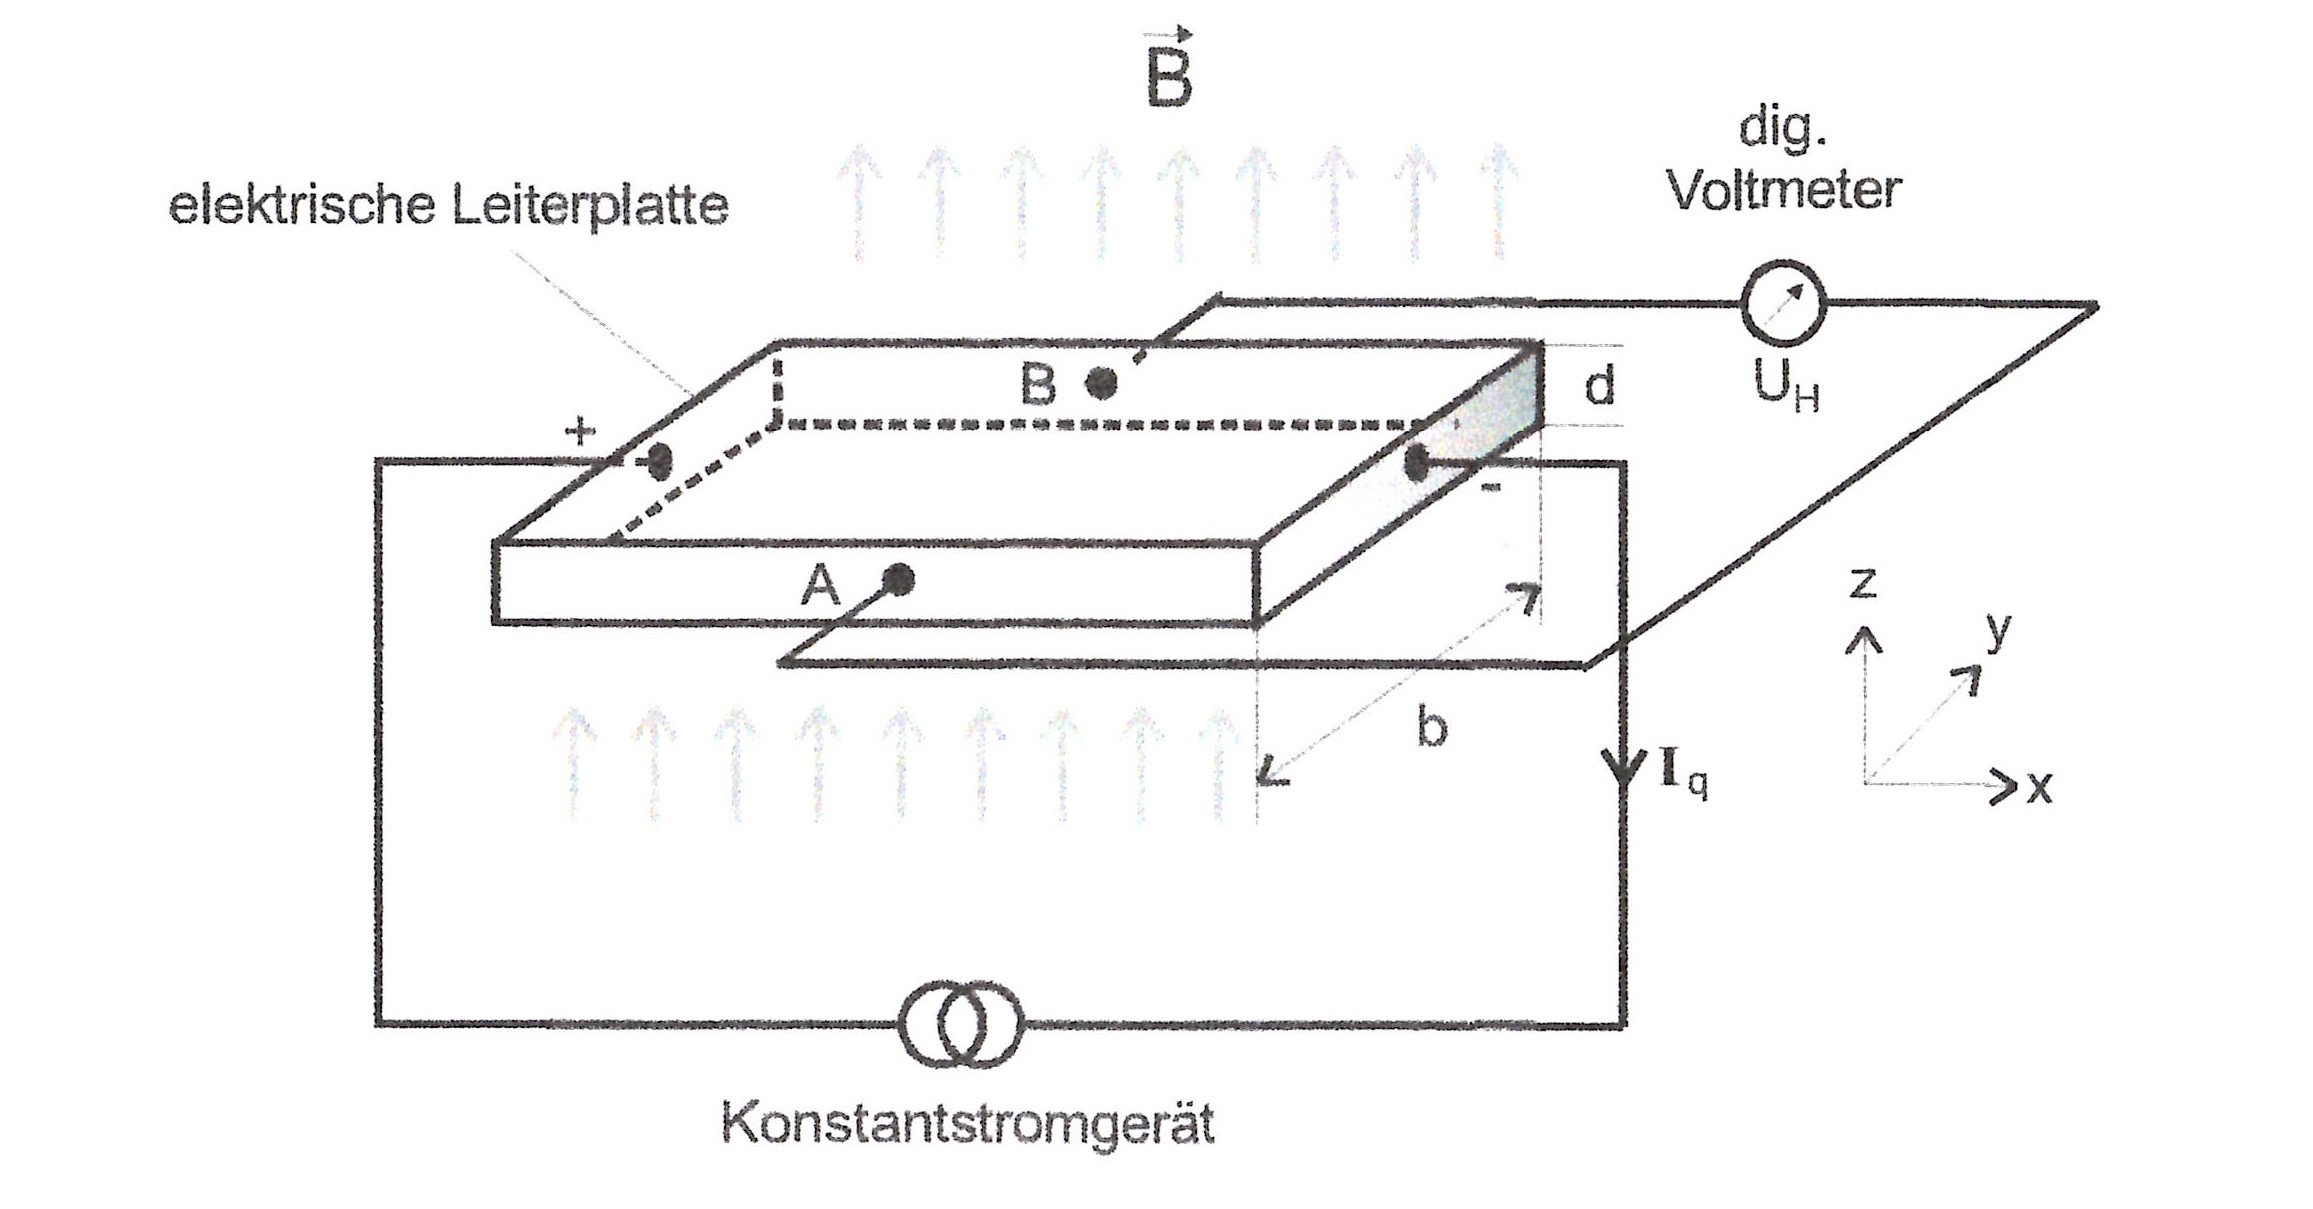
\includegraphics{Lorentz_Kraft.jpg}
  \caption{Versuchsanordnung zur Beobachtung des Hall-Effektes \cite{anleitung01}}
  \label{}
\end{figure}

\subsection{Bestimmung weiterer Leitfähigkeitsparameter}

Mit den beiden oben beschriebenen Messungen lassen sich nun also die Leitfähigkeitsparameter
$\bar{\tau}$ und $n$, sowie die Driftgeschwindigkeit $\bar{v}\ua{d}$ bestimmen.
Des weiteren soll die mittlere freie Weglänge $\bar{l}$, also die Entfernung
zwischen zwei Zusammenstößen der Stoßpartner, mit der Beziehung $\bar{l} = \bar{\tau} \cdot |v|$
bestimmt werden.

$|v|$ steht hierbei für die Totalgeschwindigkeit der Elektronen, die von der
Driftgeschwindigkeit abweicht. Sie kommt im Gegensatz zur Driftgeschwindigkeit
nicht durch ein äußeres elektrisches Feld zustande, sondern durch die Wärmebewegung
der Kristallbausteine. $|v|$ kann mithilfe der Fermi-Energie und dem Äquipartitionstheorem
bestimmt werden und führt für die mittlere freie Weglänge somit auf folgende Formel:

\begin{align}
  |\bar{v}| \approx \sqrt{\frac{2E\ua{F}}{m\ua{0}}} \\
  \bar{l} = \bar{\tau} \sqrt{\frac{2E\ua{F}}{m\ua{0}}}
\end{align}

Des weiteren soll der Proportionalitätsfaktor zwischen der Driftgeschwindigkeit
und dem angelegtem E-Feld, auch Beweglichkeit genannt, bestimmt werden :

\begin{equation}
  \vec{\bar{v}}\ua{d} = \mu\vec{E}
\end{equation}

\subsection{Elektrizitätsleitung in Metallen mit positiver Ladungsträgerdichte}

Wie am Anfang schon beschrieben, kann es teilweise vorkommen, dass sich zwei
Energienbänder überlappen. Bei einem spontanem Wechsel von Elektronen zwischen zwei
Bändern werden Lücken zurückgelassen, die ortsveränderlich sind und sich wie eine
positive Ladung verhalten. Dieser Beitrag zur elektrischen Leitfähigkeit wird
auch anormaler Hall-Effekt gennant, welcher nun ein umgekehrtes Vorzeichen besitzt
und zur Bestimmung der Ladungsträgerart verwendet werden kann.

\subsection{Messtechnische Hinweise}

Ein Problem bei der Messung der Hall-Spannung ist die fehlende Möglichkeit, die
beiden Kontaktstellen für das Multimeter auf einer Äquipotenzialebene anzuordnen.
Um die so durch den Spannungsabfall auftretende Störspannung raus zu filtern,
werden zwei Messungen angefertigt, zwischen denen das Magnetfeld einmal umgepolt
wird. Mit folgender Formel lässt sich dann die eigentliche Hall-Spannung ausrechnen:

\begin{equation}
  U\ua{H} = \frac{1}{2} \cdot ( U\ua{ges+} - U\ua{ges-} )
\end{equation}


\section{Versuchsdurchführung und Versuchsaufbau}

Als erstes wurde mithilfe eines Teslameters die magnetische Feldstärke zwischen
den beiden Spulen für verschiedene Stromstärken gemessen. Dafür wurden zwei nebeneinander
stehende Spulen in Reihe an einen Generator angeschlosse. Die Feldstärke wurde
zwischen den beiden Spulen gemessenen. Dabei wurden zwei Messungen
vorgenommen, eine bei der die Stromstärke langsam erhöht wurde und eine weitere
bei der die Stromstärke langsam gesenkt wurde, um eine Hystereskurve bestimmen
zu können.

Anschließend wurde für beide Proben der Widerstand gemessen, indem mit einem Generator
ein Strom an den Proben angelegt wurde und die Spannung mithilfe eines Multimeters
gemessen wurde. Mithilfe einer Schieblehre wurden dann
von beiden Proben die Abmessungen bestimmt.

Danach wurde die Messungen des Hall-Effektes bei der Zinkprobe vorgenommen.
Dafür wurde als  erstes der Strom, der durch die Probe fließt, konstant gelassen
und der Spulenstrom verändert. Die Probe wird dafür zwischen den beiden Spulen
befestigt. Es wurden zwei Messreihen angelegt, zwischen denen
die Magneten einmal umgepolt wurden. Anschließend wurde noch eine Messung durchgeführt,
in der der Spulenstrom konstant gelassen wurde, während der durch die Probe fließende
Strom verändert wurde.
